%\usepackage{graphicx}

\chapter{Design}\label{ch:design}

\section{User Modelling}

After reviewing the previous works in user modelling, we chose to conduct a survey similar to the ones performed in the literature to help determine whether there are certain patterns in feed preferences for users and to group those patterns into user types. For example, finding that there is a significant group of users that prefer to see friend's social updates, photos and event information, we can classify those set of preferences as a user type. 

This approach is further verified by Cle~\cite{clemmensen2004four} who had found that HCI professionals commonly used surveying as a part of user modelling.

Our survey was formulated with ideas from the survey conducted by Bon~\cite{bonds2010myspace} and will serve as the basis of our user modelling. The bulk of our survey can be seen in Figure 3.1.

\begin{center}
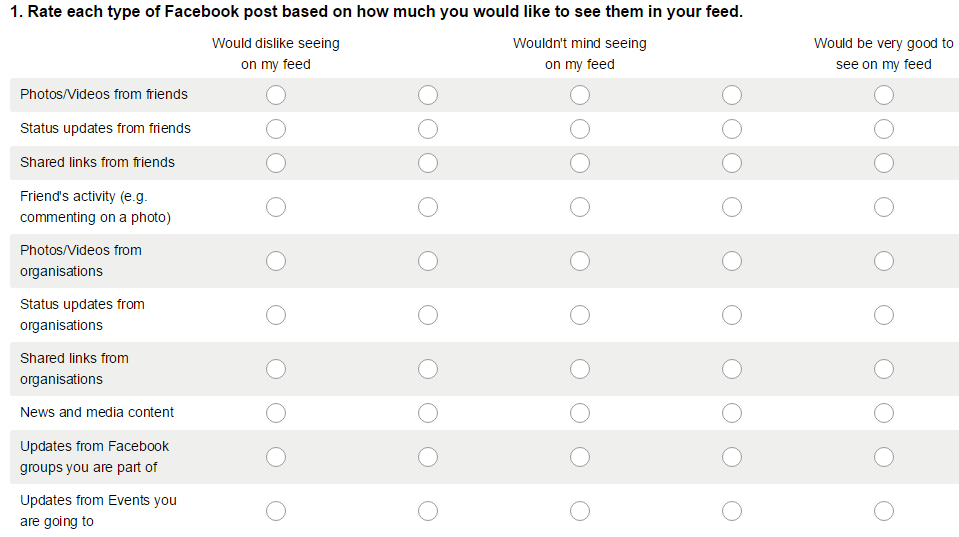
\includegraphics[scale=0.7]{images/SurveyQuestion.png}
\captionof{figure}{Survey Questions}
\end{center}

There was a possibility that the results of this survey did not yield any significant patterns, in which case we had planned to simply display the survey questions themselves in our application to give the user full customisation of their feed ranking. 
This approach was not desired as it may have discouraged users of the system due to the amount of time it may take to answer the questions. fortunately the survey did yield some significant patterns in feed preferences and the former approach could be taken, as will be explained in the implementation section.

\newpage
\section{Ranking Algorithm}

Following a review of the previous works, we have chosen to combine modules proposed from multiple papers to construct our ranking algorithm. We concluded that the main factors affecting our ranking algorithm were the following:

\begin{itemize}
	\item Topic Classification
	\item Connections
	\item Freshness
	\item Diversity
	\item User Modelling
\end{itemize}

User modelling was mentioned previously and will play a role in our algorithm. Topic Classification, Connections, Freshness and Diversity implementation will come from ideas from various algorithms suggested by works that we have researched. 

\newpage
\section{System Architecture}

\begin{center}
\includegraphics[scale=0.6]{images/newblockdiagram.png}
\captionof{figure}{Block Diagram of System}
\end{center}

In our design in Figure 3.2, we will have a front end module which will be the website (Node Authentication) that is seen by the user. The website will have a login screen for user authentication which will allow us to pull the data from their Facebook feed. Included with the login form will be a set of checkboxes indicating which user types they think they are with a brief description of each type. 

When the user logs in we note which checkboxes they had selected and the associated weights e.g. feed items from friends, feed items from news / media, etc. from the user types selected and proceed to pull the user’s feed using their credentials. Once we have the user’s feed, it is pushed through our ranking algorithm which applies the modules specified earlier in the order listed below: 

\begin{itemize}
\item The feed will be first be passed over to the freshness module. We will use Aga's~\cite{Aga2014} method and assign a decay factor depending on their time of creation. 
\item Then the topic classification module will decide which feed items contain content that the user will most likely be interested in, using the method proposed by Szo~\cite{szomszor2008semantic}.
\item After this, connection to the poster will be considered in the connections module which will simply look at how often the user has interacted with the person who posted that item and give a score based on that. This is an implementation of the solution proposed by Li~\cite{LiTiaLee2010}
\item This feed will then be re-ranked based on the new scores and passed over to the diversity module. In this module, we will re-rank the feed and add a negative score to feed items of the same type. This method was also proposed by Aga's~\cite{Aga2014}.
\item Lastly, the newly ranked feed will be displayed in the frontend website in front of the user.
\end{itemize}

It should also be noted that our application does not contain a database as we deemed it unnecessary for our purposes. All of the user’s feed items can and must be pulled via the Facebook API and there is no need to create accounts as we already need the user’s Facebook accounts to authenticate. 

Infact, our application is completely stateless, in that no data obtained is persistent and we ask the user to authenticate and select their user types for every time they wish to view their feed using our ranking. This is primarily because the incurred delay from pulling the user’s feed every time is negligible and we are only aiming to prove the effectiveness of the multiple proposed algorithms implemented in our design rather than focusing on efficiency and user experience.